\section{留数定理及其应用}

留数定理是复变函数论中的一个重要定理, 用于计算复函数在孤立奇点处的积分值. 
具体来说, 留数定理指出, 如果一个复函数在某个孤立奇点处解析 (即在该点附近可展开成幂级数), 
那么该函数在该孤立奇点处的留数就等于以该孤立奇点为中心的 Laurent 级数展开式中负幂次的系数. 

\subsection{留数}

若点 $a$ 为函数 $f(z)$ 的解析点, 存在邻域 $|z-a|<R$, $f(x)$ 在领域内解析, 这时若在邻域内作圆
$C:|z-a|=r<R$, 那么 根据 Cauchy 定理
$$\oint_{C}f(z)\dd z=0$$
若点 $b$ 为函数 $f(z)$ 的孤立奇点, 则函数在 $0<|z-b|<R$ 内解析, 这是若作圆 $C:|z-a|=r<R$, 由于
围道内有奇点, 所以 $$\oint_C f(z)\dd z\text{ 不一定为零}$$
在 $0<|z-b|<R$ 的环域内 $f(z)$ 有 Laurent 展开:
$$f(z)=\sum_{-\infty}^{+\infty}a_n(z-b)^n,~a_n=\dfrac{1}{2\pi\mathrm{i}}\oint_{|z-b|=r}\dfrac{f(z)}{(z-b)^{n+1}}\dd z$$
令 $n=-1$, 即得 $$\oint_{|z-b|=r}f(z)\dd z=2\pi\mathrm{i}a_{-1}.$$

\begin{definition}[留数]
    若 $b$ 为 $f(z)$ 的孤立奇点, 定义函数 $f(z)$ 在孤立奇点 $b$ 的留数等于 $f(z)$ 在 $b$ 的空心邻域内 Laurent
    展开式中 $(z-b)^{-1}$ 幂的系数 $a_{-1}$, 并记作 $\Res[f(b)].$
\end{definition}

\subsection{留数定理}

如果我们要计算一闭合围道积分 $\displaystyle\oint_{C}f(z)\dd z$, 假设闭合围道内部, 被积函数除有限几个孤立奇点 $b_k$, 
根据复连通区域 Cauchy 定理, 作小圆 $\gamma_1,\gamma_2,\cdots,\gamma_{n}$ 将每个奇点包围, 则
$$\oint_{C}f(z)\dd z=\sum_{k=1}^{n}\oint_{\gamma_k}f(z)\dd z=2\pi\i\sum_{k=1}^{n}\Res[f(b_k)].$$

\begin{figure}[H]
    \centering
    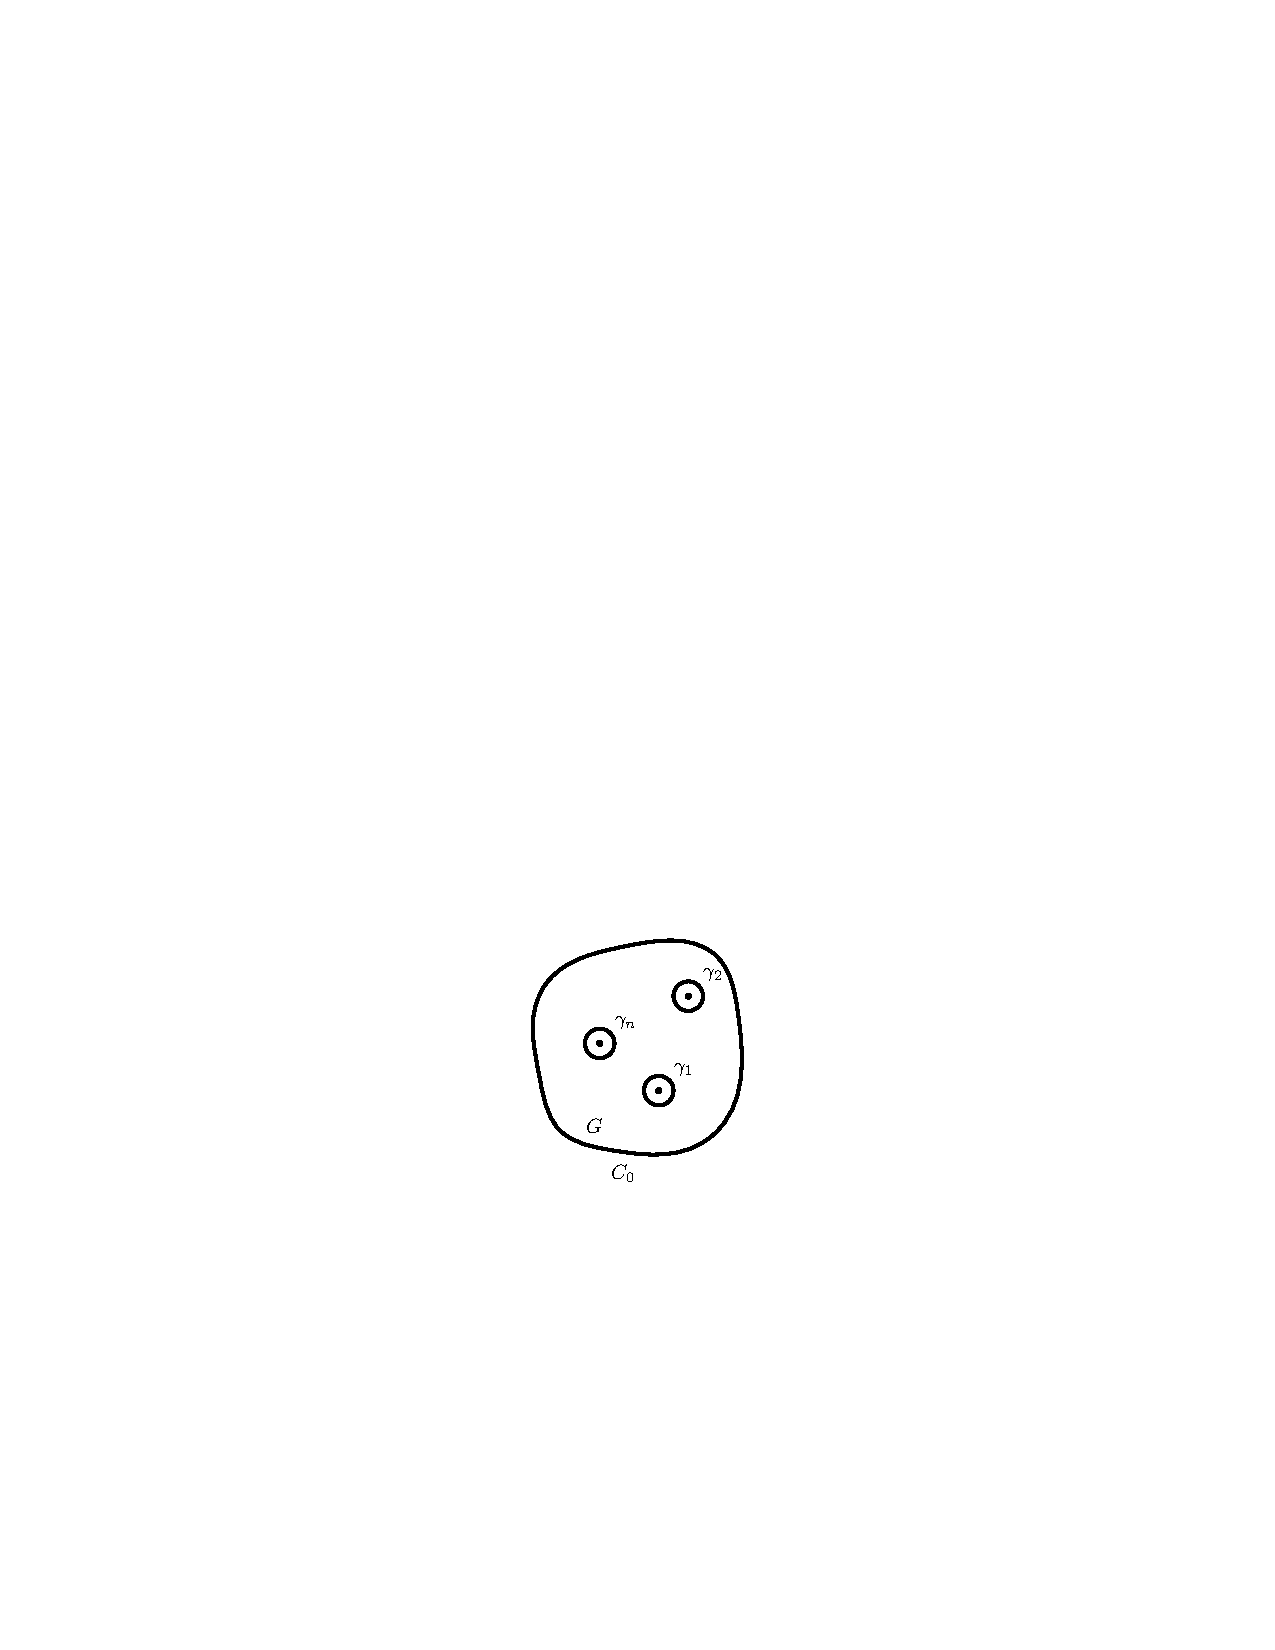
\includegraphics{figures/liushu1.pdf}
    \caption{}
\end{figure}

\begin{theorem}[留数定理]
    \index{留数定理}设 $C$ 为简单闭合围道, $G$ 为 $C$ 的内区域, 若除 $G$ 内有限个孤立奇点 $b_k$, $k=1,2,\dots,n$ 外, 函数在 $\overline{G}$ 内解析, 则
    $$\oint_{C}f(z)\dd z=2\pi\i\sum_{k=1}^{n}\Res[f(b_k)].$$
\end{theorem}

\subsection{留数计算}

\subsubsection{一阶极点}

在 $b$ 点的某一空心邻域内 $$f(z)=\dfrac{1}{z-b}\phi(z)$$
$\phi(z)$ 在含中心 $b$ 点的邻域内解析, $\phi(b)\neq 0$, 作 Taylor 展开 $$\phi(z)=\sum_{n=0}^{+\infty}\alpha_n(z-b)^n$$
于是 $$\Res[f(b)]=\alpha_0=\phi(b)$$
由连续性 $$\Res[f(b)]=\lim_{z\to b}(z-b)f(z)$$

特别常见的情况, 当 $f(z)=\dfrac{P(z)}{Q(z)}$, $P(z)$ 和 $Q(z)$ 在 $b$ 点及其邻域内解析, $b$ 是 $Q(z)$ 的一阶零点, $P(b)\neq0$, 则
$$\Res[f(b)]=\lim_{z\to b}(z-b)\dfrac{P(z)}{Q(z)}=P(b)\lim_{z\to b}\dfrac{z-b}{Q(z)}\xlongequal[]{L'}\dfrac{P(b)}{Q'(b)}$$

\subsubsection{高阶极点}

设 $z=b$ 是 $f(z)$ 的 $m$ 阶极点 $$f(z)=(z-b)^{-m}\phi(z)$$
$\phi(z)$ 在 $b$ 的某个邻域内解析 $$\phi(z)=\sum_{n=0}^{+\infty}\alpha_n(z-b)^n$$
$\phi(b)\neq0$, 则 $$\Res[f(b)]=\alpha_{m-1}=\dfrac{1}{(m-1)!}\phi^{(m-1)}(b)$$
将 $b$ 换成极限 $z\to b$, 有
$$\Res[f(b)]=\dfrac{1}{(m-1)!}\lim_{z\to b}\dv[m-1]{\qty[(z-b)^mf(z)]}{z}.$$

\subsubsection{本性奇点或高阶极点}

对于本性奇点时只能求 Laurent 展开系数 $a_{-1}$.

对于高阶极点, 很多情况下求展开系数往往比用高阶极点的留数公式简单, 对于 $m$ 阶极点即求 $\phi(z)=(z-b)^mf(z)$ 的 Taylor 展开系数 $a_{m-1}$.

\begin{example}
    函数 $f(z)=\dfrac{\e^{\i z}}{z\qty(z^2+1)^2}$, 求 $\Res[f(z)].$
\end{example}
\begin{solution}
    函数在 $z=\i$ 有二阶极点, 这时
    $$\phi(z)=(z-\i)^2\dfrac{\e^{\i z}}{z\qty(z^2+1)^2}=\dfrac{\e^{\i z}}{z(z+\i)^2}$$
    要求 $m-1=1$ 次项的系数 $\alpha_1$, 用待定系数法, 令 $z-\i=t$, 于是
    $$(t+\i)(t+2\i)^2\sum_{n=0}^{\infty}\alpha_nt^n=\e^{\i(t+\i)}=\e^{-1}\sum_{n=0}^{\infty}\dfrac{\i^n}{n!}t^n$$
    即 $$(-4\i-8t+\cdots)\sum_{n=0}^{\infty}\alpha_nt^n=\e^{-1}\sum_{n=0}^{\infty}\dfrac{\i ^n}{n!}t^n$$
    先比较两边 $0$ 次项系数 $$-4\i \alpha_0=\e^{-1}$$
    得 $\alpha_0=\dfrac{\i}{4\e}$, 再比较两边 1 次项系数 $$-4\i\alpha_1-8\alpha_0=\dfrac{\i}{\e}$$
    得 $\alpha_1=-\dfrac{3}{4\e}$, 所以 $$\Res[f(i)]=-\dfrac{3}{4\e}.$$
\end{solution}

\subsection{留数定理的应用}

\subsubsection{有理三角函数的积分}

考虑积分 $\displaystyle I=\int_{0}^{2\pi}R(\cos\theta,\sin\theta)\dd \theta$, 其中 $R$ 是 $\cos\theta,~\sin\theta$ 的有理函数, 作变换
$$z=\e^{\i\theta},~\cos\theta=\dfrac{z+z^{-1}}{2}=\dfrac{z^2+1}{2z},~\sin\theta=\dfrac{z-z^{-1}}{2\i}=\dfrac{z^2-1}{2\i z},~\dd \theta=\dfrac{\dd z}{\i z}$$
积分路径变换为 $z$ 平面上的单位圆 $|z|=1$, 于是
$$I=\oint_{|z|=1}R\qty(\dfrac{z^2+1}{2z},\dfrac{z^2-1}{2\i z})\dfrac{\dd z}{\i z}=2\pi\sum_{|z|<1}\Res[\dfrac{1}{z}R\qty(\dfrac{z^2+1}{2z},\dfrac{z^2-1}{2\i z})].$$

\begin{example}
    计算积分 $\displaystyle I=\int_{0}^{2\pi}\dfrac{\dd \theta}{1+\varepsilon\cos\theta}~  |\varepsilon|<1.$
\end{example}
\begin{solution}
    作变换 $z=\e^{\i\theta}$, 那么有
    \begin{flalign*}
        I=\oint_{|z|=1}\dfrac{1}{1+\varepsilon\dfrac{z^2+1}{2z}}\dfrac{\dd z}{\i z}=\dfrac{1}{\i}\oint_{|z|=1}\dfrac{2}{\varepsilon z^2+2z+\varepsilon}\dd z=2\pi\sum_{|z|<1}\Res[\dfrac{2}{\varepsilon z^2+2z+\varepsilon}]
    \end{flalign*}
    解方程 $\varepsilon z^2+2z+\varepsilon=0$, 可得被积函数两个一阶极点为
    $$z_{1,2}=\dfrac{-1\pm\sqrt{1-\varepsilon^2}}{\varepsilon}$$
    其中 $|z_1|<1,~|z_2|>1$, 于是
    \begin{flalign*}
        I=2\pi\Res[\dfrac{2}{\varepsilon z^2+2z+\varepsilon}]_{z=z_1}=2\pi\dfrac{2}{2\varepsilon z+2}\biggl |_{z=z_1}=\dfrac{2\pi}{\sqrt{1-\varepsilon^2}}.
    \end{flalign*}
\end{solution}

\begin{example}
    计算积分 $\displaystyle\int_{0}^{2\pi}\dfrac{\dd \theta}{1+\cos^2\theta}.$
\end{example}
\begin{solution}
    由 $\cos \theta=\dfrac{z^2+1}{2z},~\dd \theta=\dfrac{\dd z}{\i z}$, 于是原式等价为
    $$I=\oint_{\Gamma:|z|=1}\dfrac{4z\dd z}{\i\qty(z^4+6z^2+1)}\xlongequal{z^2=u}\dfrac{4}{\i}\oint_{\Gamma}\dfrac{\dd u}{u^2+6u+1}=2\pi\i\cdot\Res[\dfrac{4}{\i}f\qty(-3+2\sqrt{2})]=\sqrt{2}\pi.$$
    将 $z^2=u$ 替换后, 当 $z$ 绕 $\Gamma$ 一周时, $u$ 亦在其上绕二周.
\end{solution}

\begin{example}
    计算 $\displaystyle I=\int_{0}^{2\pi}\dfrac{\cos2\theta}{5-4\cos\theta}\dd \theta.$
\end{example}
\begin{solution}
    由 $\cos2\theta=\dfrac{1}{2}\qty(z^2+z^{-2}),~\cos\theta=\dfrac{1}{2}\qty(z+z^{-1}),~\dd \theta=\dfrac{\dd z}{\i z}$, 于是 
    \begin{flalign*}
        I=\oint_{|z|=1}\dfrac{\dfrac{1}{2}\qty(z^2+z^{-2})}{5-2\qty(z+z^{-1})}\dfrac{\dd z}{\i z}=\dfrac{\i }{4}\oint_{|z|=1}\dfrac{\qty(z^4+1)\dd z}{z^2\qty(z-\dfrac{1}{2})(z-2)}=-\dfrac{\pi}{2}\sum_{\text{上半平面}}\Res[f(z)]
    \end{flalign*}
    其中 $f(z)=\dfrac{\qty(z^4+1)}{z^2\qty(z-\dfrac{1}{2})(z-2)}$, 那么有
    $$\Res[f(0)]=\dfrac{1}{1!}\lim_{z\to0}\dv{z}\qty[z^2\cdot\dfrac{\qty(z^4+1)}{z^2\qty(z-\dfrac{1}{2})(z-2)}]=\dfrac{5}{2},~\Res[f\qty(\dfrac{1}{2})]=\dfrac{z^4+1}{z^2(z-2)}\biggl |_{z=\frac{1}{2}}=-\dfrac{17}{6}$$
    于是 $I=-\dfrac{\pi}{2}\qty(-\dfrac{17}{6}+\dfrac{5}{2})=\dfrac{\pi}{6}.$
\end{solution}

\begin{example}
    计算 $\displaystyle I=\int_{0}^{\pi}\dfrac{\cos m\theta}{5-4\cos\theta}\dd \theta$, $m$ 是正整数.
\end{example}
\begin{solution}
    积分号下的函数为 $x$ 的偶函数, 故 $\displaystyle I=\dfrac{1}{2}\int_{-\pi}^{\pi}\dfrac{\cos m\theta}{5-4\cos\theta}\dd \theta$, 令 
    $$I_1=\int_{-\pi}^{\pi}\dfrac{\cos m\theta}{5-4\cos\theta}\dd \theta,~I_2=\int_{-\pi}^{\pi}\dfrac{\sin m\theta}{5-4\cos\theta}\dd \theta$$
    故有 $$I_1+\i I_2=\int_{-\pi}^{\pi}\dfrac{\e^{\i m\theta}}{5-4\cos\theta}\dd \theta=\dfrac{\i}{2}\oint_{|z|=1}\dfrac{z^m}{\qty(z-\dfrac{1}{2})(z-2)}\dd z$$
    并且在圆周内部仅有一个一阶极点 $z=\dfrac{1}{2}$, 于是 
    $$\Res[\dfrac{z^m}{z-2}]_{z=\frac{1}{2}}=-\dfrac{1}{3\cdot 2^{m-1}}$$
    由留数定理, $$I_1+\i I_2=2\pi\i\cdot\dfrac{\i}{2}\cdot\dfrac{1}{-3\cdot 2^{m-1}}=\dfrac{\pi}{3\cdot 2^{m-1}}$$
    知 $$I_1=\dfrac{\pi}{3\cdot 2^{m-1}},~I_2=0$$
    故所求积分 $I=\dfrac{1}{2}I_1 =\dfrac{\pi}{3\cdot 2^m}.$
\end{solution}

\subsubsection{有理函数无穷积分}

考虑积分 $\displaystyle I=\int_{-\infty}^{+\infty}R(x)\dd x$, 其中 $R(x)$ 为有理函数, 无穷积分定义为
$$\int_{-\infty}^{+\infty}f(x)\dd x=\lim_{\substack{R_1\to+\infty\\R_2\to+\infty}}\int_{-R_1}^{R_2}f(x)\dd x$$
对于有理函数 $R(x)=P_n(x)/Q_m(x)$, 只有当分母多项式 $Q_m(x)$ 次数比分子多项式 $P_n(x)$ 次数至少大 2 时积分存在 $$m-n\geqslant 2$$
若积分存在, 则 $$I=\lim_{R\to+\infty}\int_{-R}^{R}R(x)\dd x$$

计算 $\displaystyle\int_{-R}^{R}R(x)\dd x$, 从复平面上看, 这是一个沿实轴的复变积分, 为应用留数定理, 必须先构造适当的围道, 
我们补上以原点为圆心, $R$ 为半径的上半圆 $C_R$, 如图 \ref{figure:lsdlCR} 所示.

\begin{minipage}[b]{0.45\linewidth}
    \begin{figure}[H]
        \centering
        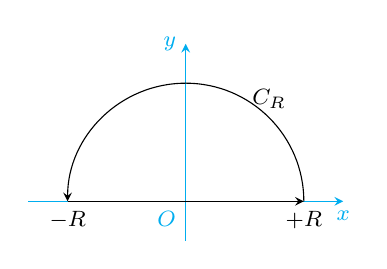
\begin{tikzpicture}[->,samples=100,>=stealth,font=\footnotesize]
            \draw[->,cyan](-2,0)--(0,0)node[below left]{$O$}--(2,0)node[below]{$x$};
            \draw[->,cyan](0,-0.5)--(0,2)node[left]{$y$};
            \draw[black] (1.5,0) arc (0:180:1.5)node[above,near start]{$C_R$};
            \draw[black] (-1.5,0)--(1.5,0);
            \node[below] at (-1.5,0) {$-R$};
            \node[below] at (1.5,0) {$+R$};
        \end{tikzpicture}
        \caption{}
        \label{figure:lsdlCR}
    \end{figure}
\end{minipage}\hfill
\begin{minipage}[b]{0.45\linewidth}
    \begin{figure}[H]
        \centering
        \begin{tikzpicture}[->,samples=100,>=stealth,font=\footnotesize]
            \draw[->,cyan](-2,0)--(0,0)node[below left]{$O$}--(2,0)node[below]{$x$};
            \draw[->,cyan](0,-2)--(0,2)node[left]{$y$};
            \draw[black] (1.5,0) arc (0:180:1.5)node[above,near start]{$C_R$};
            \draw[black] (-1.5,0)--(1.5,0);
            \node[below] at (-1.5,0) {$-R$};
            \node[below] at (1.5,0) {$+R$};
            \node[left] at (0,1) {$\mathrm{i}$};\draw[fill=black] (0,1) circle (0.5pt);
            \node[left] at (0,-1) {$\mathrm{i}$};\draw[fill=black] (0,-1) circle (0.5pt);
        \end{tikzpicture}
        \caption{}
        \label{liushu3}
    \end{figure}
\end{minipage}

于是 $$\oint_C R(z)\dd z=\int_{-R}^{R}R(x)\dd x+\int_{C_R}R(z)\dd z$$
任何有理函数只有有限个的孤立奇点, 所以 $R(z)$ 在上半平面只有有限个孤立奇点, $R$ 足够大时, 则围道包围上半平面所有的奇点, 由留数定理又有
$$\oint_CR(z)\dd z=2\pi\i\sum_{\text{上半平面}}\Res[R(z)]$$
对于无穷积分存在的有理函数 $R(z)$, 满足分母多项式次数比分子多项式次数至少大 2, 则
$$\lim_{z\to\infty}zR(z)=\lim_{z\to\infty}z\dfrac{P_n(x)}{Q_m(z)}=0$$
由大圆弧定理 $$\lim_{R\to\infty}\int_{C_R}R(z)\dd z=0$$
于是 $$\int_{-\infty}^{+\infty}R(x)\dd x=2\pi\i\sum_{\text{上半平面}}\Res[R(z)]$$

\begin{example}
    计算积分 $\displaystyle I=\int_{-\infty}^{+\infty}\dfrac{\dd x}{\qty(1+x^2)^3}.$
\end{example}
\begin{solution}
    令 $f(x)=\dfrac{1}{\qty(1+x^2)^3},~\displaystyle I=\lim_{R\to\infty}\int_{-R}^{R}f(x)\dd x $, 考虑围道如图 \ref{liushu3} 所示, 
    则有
    \begin{flalign*}
        \oint_Cf(z)\dd z & =\int_{-R}^{R}f(x)\dd x+\int_{C_R}f(z)\dd z=2\pi\i\sum_{\text{上半平面}}\Res[R(z)]=2\pi\i\Res[f(i)]                                                                                                     \\
                         & =2\pi\i\cdot \dfrac{1}{2!}\lim_{z\to\i}\dv[2]{\qty[(z-\i)^3\dfrac{1}{\qty(1+z^2)^3}]}{z}=2\pi\i\cdot\dfrac{1}{2}\dv[2]{(z+\i)^{-3}}{z}\biggl |_{z=\i}=2\pi\i\cdot\qty(-\dfrac{3}{16}\i)=\dfrac{3\pi}{8}
    \end{flalign*}
    因为 $\displaystyle \lim_{z\to\infty}z\cdot\dfrac{1}{\qty(1+z^2)^3}=0$, 由大圆弧定理 $$\lim_{R\to\infty}\int_{C_R}f(z)\dd z=\i\pi\cdot0=0$$
    于是原积分等于 $\dfrac{3\pi}{8}.$
\end{solution}

\begin{example}
    计算反常积分 $\displaystyle I=\int_{-\infty}^{+\infty}\dfrac{\dd x}{\qty(x^2+x+1)^2}.$
\end{example}
\begin{solution}
    令 $f(x)=\dfrac{1}{\qty(x^2+x+1)^2},~\displaystyle I=\lim_{R\to\infty}\int_{-R}^{R}f(x)\dd x$, 则有 $z_{1,2}=\dfrac{-1\pm\sqrt{3}\i}{2}$, 于是
    \begin{flalign*}
        \oint_Cf(z)\dd z & =\int_{-R}^{R}f(x)\dd x+\int_{C_R}f(z)\dd z=2\pi\i\sum_{\text{上半平面}}\Res[f(z)]=2\pi\i\Res[f(z_1)]                                                                        \\
                         & =2\pi\i\cdot\dfrac{1}{1!}\lim_{z\to z_1}\dv{z}\qty[(z-z_1)^2\dfrac{1}{\qty(z^2+z+1)^2}]=2\pi\i\cdot\dv{z}\qty(z-\overline{z}_1)^{-2}\biggl |_{z=z_1}=\dfrac{4\pi}{3\sqrt{3}}
    \end{flalign*}
    因为 $\displaystyle\lim_{z\to\infty}z\cdot f(z)=0$, 由大圆弧定理 $\displaystyle\lim_{R\to\infty}\int_{C_R}f(z)\dd z=0$, 故原积分等于 $\dfrac{4\pi}{3\sqrt{3}}.$
\end{solution}

\subsubsection{含三角函数的无穷积分}

考虑积分 $\displaystyle I=\int_{-\infty}^{+\infty}R(x)\mathrm{e}^{\i px}\dd x,~p>0$, 其中 $R(x)$ 为有理函数, 积分的实部和虚部分别为
$$\Re I=\int_{-\infty}^{+\infty}R(x)\cos px\dd x,~\Im I=\int_{-\infty}^{+\infty}R(x)\sin px\dd x$$
当且仅当有理函数 $R(x)=P_n(x)/Q_m(x)$ 的分母多项式 $Q_m(x)$ 次数比分子多项式 $P_n(x)$ 的次数大 1 时无穷积分存在.
$$m-n\geqslant 1$$

对于积分 $I$ 同样考虑围道积分 $$\oint_{C}R(x)\e^{\i pz}\dd z=\int_{-R}^{R}R(x)\e^{\i px}\dd x+\int_{C_R}R(z)\e^{\i pz}\dd z=2\pi\i\sum_{\text{上半平面}}\Res[R(x)\e^{\i pz}]$$

\begin{lemma}[Jordan 引理]
    设在 $0\leqslant \arg z\leqslant \pi$ 的范围内, 当 $|z|\to\infty$ 时, $Q(z)$ 一致地趋近于 0, 则 
    $$\lim_{R\to\infty}\int_{C_R}Q(z)\e^{\i pz}\dd z=0$$
    其中 $p>0,C_R$ 是以原点为圆心, $R$ 为半径的上半圆.
\end{lemma}

对于 $R(z)$, 满足分母多项式次数比分子多项式次数至少大 1, 则
$$\lim_{z\to\infty}R(z)=\lim_{z\to\infty}\dfrac{P_n(z)}{Q_m(z)}=0$$
由 Jordan 引理 $$\lim_{R\to\infty}\int_{C_R}R(z)\e^{\i pz}\dd z=0$$
于是 $$\int_{-\infty}^{+\infty}R(z)\e^{\i px}\dd x=2\pi\i\sum_{\text{上半平面}}\Res[R(z)\e^{\i pz}].$$

\begin{example}
    计算积分 $\displaystyle I=\int_{0}^{+\infty}\dfrac{x\sin x}{x^2+a^2}\dd x,~a>0.$
\end{example}
\begin{solution}
    令 $f(x)=\dfrac{x}{x^2+a^2}$, 因为被积函数 $f(x)\sin x$ 为偶函数
    $$\int_{0}^{+\infty}f(x)\sin x\dd x=\dfrac{1}{2}\int_{-\infty}^{+\infty}f(x)\sin x\dd x=\dfrac{1}{2}\Im\int_{-\infty}^{+\infty}f(x)\e^{\i x}\dd x$$
    考虑围道积分
    $$\oint_{C}f(z)\e^{\i z}\dd z=\int_{-R}^{R}f(x)\e^{\i x}\dd x+\int_{C_R}f(z)\e^{\i z}\dd z=2\pi\i\sum_{\text{上半平面}}\Res[f(z)\e^{\i z}]$$
    易知, $z=a\i$ 为上半平面的唯一奇点, 且为一阶极点
    $$\Res[\dfrac{z\e^{\i z}}{z^2+a^2}]=\dfrac{z\e^{\i z}}{2z}\biggl |_{z=\i a}=\dfrac{1}{2}\e^{-a}$$
    所以 $$\int_{-R}^{R}f(x)\e^{\i x}\dd x+\int_{C_R}f(z)\e^{\i z}\dd z=\pi\e^{-a}\i$$
    因为 $\displaystyle\lim_{z\to\infty}f(z)=0$, 由 Jordan 引理 $\displaystyle\lim_{R\to\infty}\int_{C_R}f(z)\e^{\i z}\dd z=0$, 
    于是 $\displaystyle\int_{-\infty}^{+\infty}f(x)\e^{\i x}\dd x=\pi\e^{-a}\i$, 
    于是 $$I=\dfrac{1}{2}\Im\pi\e^{-a}\i=\dfrac{\pi}{2}\e^{-a}.$$
\end{solution}

\begin{example}
    计算反常积分 $\displaystyle I=\int_{0}^{+\infty}\dfrac{\cos x}{\qty(1+x^2)^3}\dd x.$
\end{example}
\begin{solution}
    令 $f(x)=\dfrac{1}{\qty(1+x^2)^3}$, 那么 $f(x)\cos x$ 为偶函数, 于是
    $$I=\dfrac{1}{2}\int_{-\infty}^{+\infty}f(x)\cos x\dd x=\dfrac{1}{2}\Re\int_{-\infty}^{+\infty}f(x)\e^{\i x}\dd x$$
    考虑围道积分
    $$\oint_Cf(z)\e^{\i z}\dd z=\int_{-R}^{R}f(x)\e^{\i x}\dd x+\int_{C_R}f(z)\e^{\i z}\dd z=2\pi\i\sum_{\text{上半平面}}\Res[f(z)\e^{\i z}]$$
    易知, $z=\i$ 为上半平面的唯一奇点, 且为三阶极点, 于是
    $$\phi(z)=(z-\i)^3\dfrac{\e^{\i z}}{\qty(1+z^2)^3}=\dfrac{\e^{\i z}}{(z+\i)^3}$$
    要求系数 $\alpha_2$, 用待定系数法, 令 $z-\i=t$, 于是
    $$(t+2\i )^3\sum_{n=0}^{\infty}\alpha_nt^n=\e^{\i(t+\i)}=\e^{-1}\sum_{n=0}^{\infty}\dfrac{\i ^n}{n!}t^n$$
    即 $$\qty(-8\i-12t+6\i t^2+\cdots)\sum_{n=0}^{\infty}\alpha_nt^n=\e^{-1}\sum_{n=0}^{\infty}\dfrac{\i ^n}{n!}t^n$$
    先比较两边 0 次项系数 $$-8\i\alpha_0=\e^{-1}$$
    得 $\alpha_0=\dfrac{\i}{8\e}$, 再比较两边 1 次项的系数 $$-8\i\alpha_1-12\alpha_0=\dfrac{\i}{\e}$$
    得 $\alpha_1=-\dfrac{5}{16\e}$, 再比较两边 2 此项的系数 $$-8\i \alpha_2-12\alpha_1+6\i\alpha_0=-\dfrac{1}{2\e}$$
    解得 $\alpha_2=-\dfrac{7\i}{16\e}$, 即 $$\Res[f(z)\e^{\i z}]=-\dfrac{7\i}{16\e}$$
    所以 $$\int_{-R}^{R}f(x)\e^{\i x}\dd x+\int_{C_R}f(z)\e^{\i z}\dd z=\dfrac{7\pi}{8\e}$$
    $\displaystyle\lim_{z\to\infty}f(z)=0$, 由 Jordan 引理 $\displaystyle\lim_{R\to\infty}\int_{C_R}f(z)\e^{\i z}\dd z=0$, 
    于是 $\displaystyle\int_{-\infty}^{+\infty}f(x)\e^{\i x}\dd x=\dfrac{7\pi}{8\e}$, 于是
    $$I=\Re\dfrac{1}{2}\cdot\dfrac{7\pi}{8\e}=\dfrac{7\pi}{16\e}.$$
\end{solution}

\subsubsection{实轴上有奇点的情形}

设被积函数在实轴上有奇点, 则积分 $\displaystyle\int_{-\infty}^{+\infty}f(x)\dd x$ 为瑕积分, 假设瑕点为 $c$, 
瑕积分定义为:
存在一点 $c$ 及邻域 $(\delta_1,\delta_2)$, 有 
$$\int_{a}^{b}f(x)\dd x=\lim_{\delta_1\to0}\int_{a}^{c-\delta_1}f(x)\dd x+\lim_{\delta_2}\int_{c+\delta_2}^{b}f(x)\dd x$$
如果这两个极限都不存在, 但是 $\displaystyle\lim_{\delta\to0}\qty[\int_{a}^{c-\delta}f(x)\dd x+\int_{c+\delta}^{b}f(x)\dd x]$ 存在, 定义瑕积分的主值为:
$$\vp\int_{a}^{b}f(x)\dd x=\lim_{\delta\to0}\qty[\int_{a}^{c-\delta}f(x)\dd x+\int_{c+\delta}^{b}f(x)\dd x]$$
当然, 如果瑕积分存在, 则主值也存在, 且它们一定相等, 所以, 我们考虑
$$I=\vp\int_{-\infty}^{+\infty}f(x)\dd x=\lim_{\substack{R\to\infty\\\delta\to0}}\qty[\int_{-R}^{c-\delta}f(x)\dd x+\int_{c+\delta}^{R}f(x)\dd x]$$
因为实轴上 $c$ 点是被积函数的奇点, 必须绕过奇点来构成闭合的积分围道, 如图 \ref{liushu4} 所示.

$$\oint_{C}f(z)\dd z=2\pi\i\sum_{\text{一二象限}}\Res[f(z)]=\int_{-R}^{c-\delta}f(x)\dd x+\int_{C_\delta}f(z)\dd z+\int_{c+\delta}^{R}f(x)\dd x+\int_{C_R}f(z)\dd z$$
\begin{figure}[H]
    \centering
    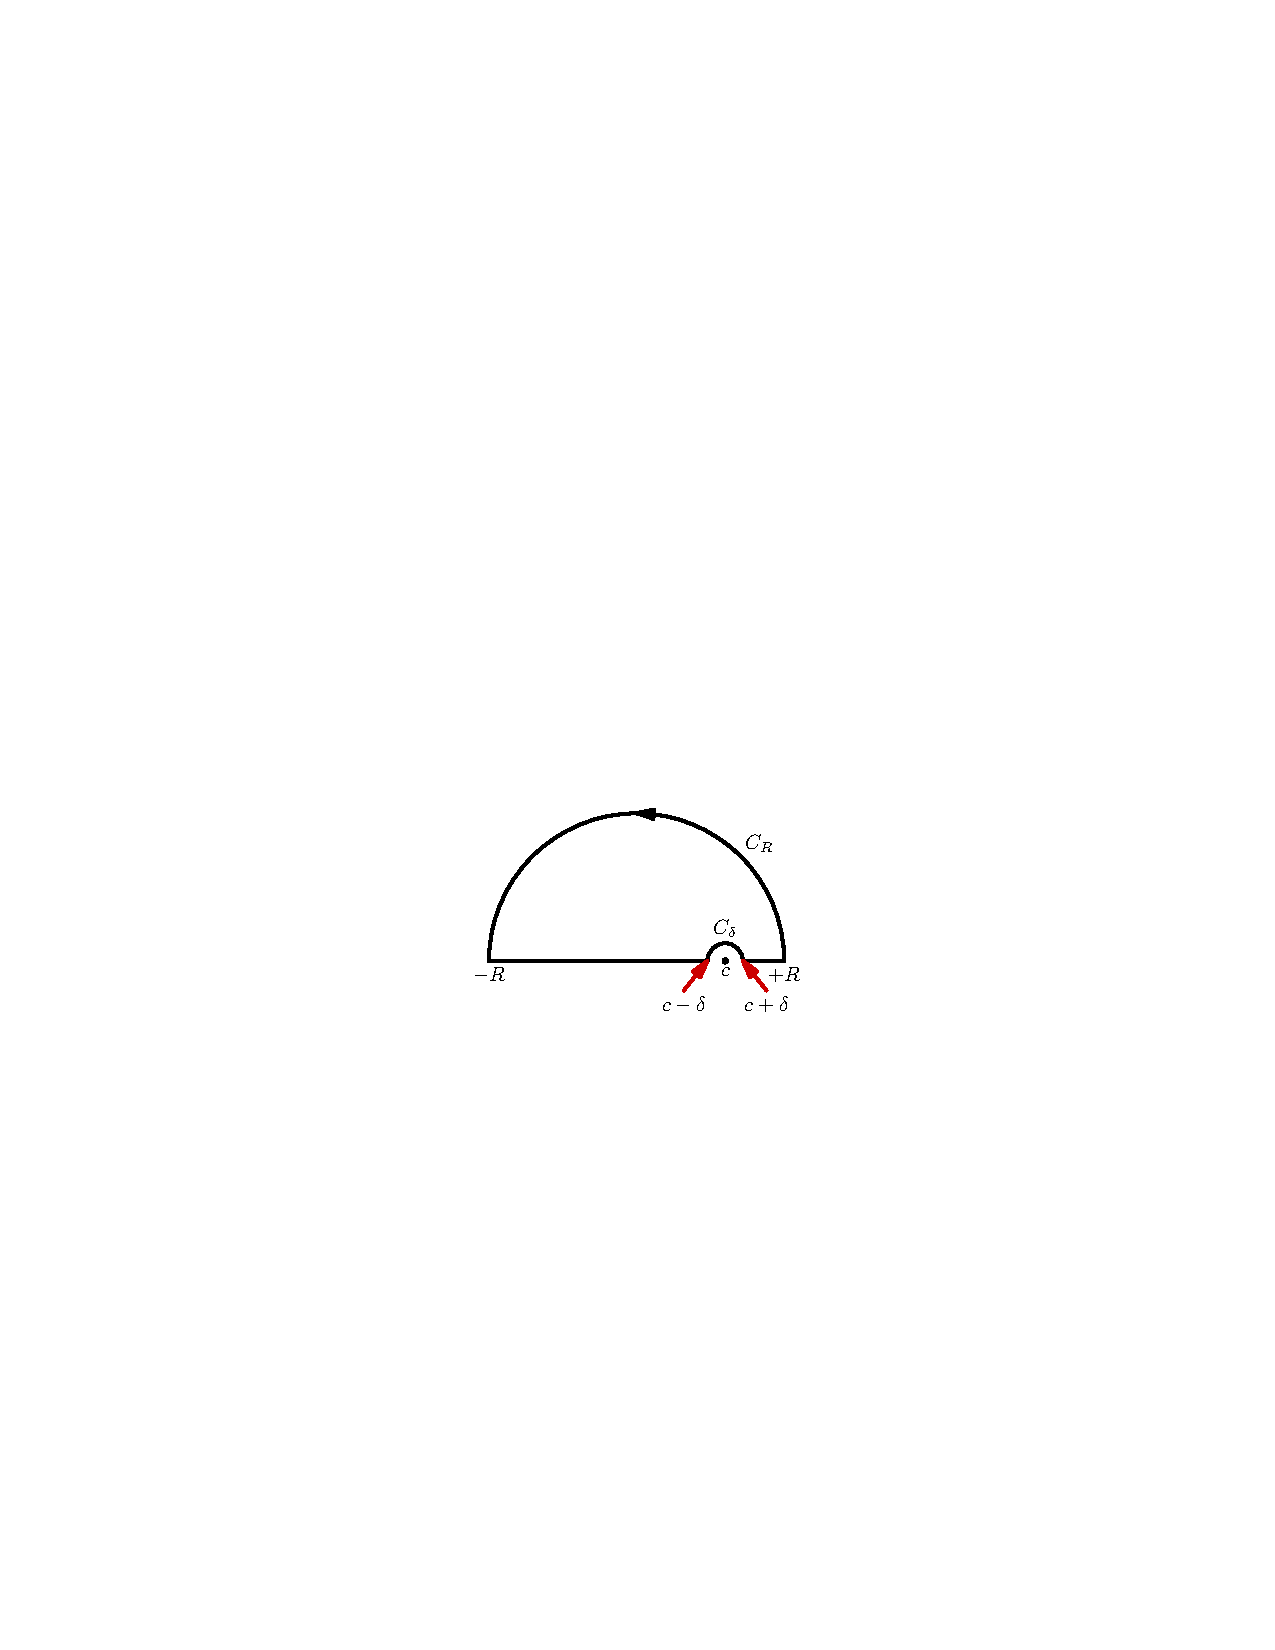
\includegraphics{figures/liushu4.pdf}
    \caption{}
    \label{liushu4}
\end{figure}
对于大圆弧积分, 我们可以用大圆弧定理或 Jordan 引理处理, 对于小圆弧 $C_\delta$ 的积分, 则需要用到小圆弧定理. 
% TODO: 实轴上有奇点的情形
